\documentclass[class=jsarticle, crop=false, dvipdfmx, fleqn]{standalone}
%% preamble for Numerical-structure-analysis report

\input{/Users/User/Documents/Project/TeX/preamble/mypreamble}

%% titles
\title{先端データ解析論 レポート}
\author{37-196360 \quad 森田涼介}


%% setting for listings
\newtcbinputlisting[auto counter]{\reportlisting}[3][]{%
	listing file = {#3},
	listing options = {language=python, style=tcblatex, numbers=left, numberstyle=\tiny},
	listing only,
	breakable,
	toprule at break = 0mm,
	bottomrule at break = 0mm,
	left = 6mm,
	sharp corners,
	drop shadow,
	title = Listings \thetcbcounter : \texttt{#2},
	label = #1,
	}



%% title format
\usepackage{titlesec}
\titleformat{\section}{\LARGE}{宿題\thesection}{0zw}{}
\newcommand{\sectionbreak}{\clearpage}
\titleformat{\subsection}{\Large}{\Alph{subsection})}{0zw}{}

\begin{document}
\section{}

線形モデル
\begin{equation}
    f_{\bm{\theta}} (\bm{x}) = \bm{\theta}^\mathrm{T} \bm{x} + \theta_0
\end{equation}
に対し,
クラス比重み付き最小二乗法を実装する。

クラス比の推定値は,
\begin{align}
    & \tilde{\pi} = \frac{\hat{A}_{+1, -1} - \hat{A}_{-1, -1} - \hat{b}_{+1} + \hat{b}_{-1}}{2 \hat{A}_{+1, -1} - \hat{A}_{+1, +1} - \hat{A}_{-1, -1}} \\
    & \hat{\pi} = \min(1,\ \max(0,\ \tilde{\pi}))
\end{align}
ここで,
\begin{align}
    & \hat{A}_{y,\ \tilde{y}} = \frac{1}{n_y n_{\tilde{y}}} \sum_{i: y_i = y} \sum_{\tilde{i}: y_{\tilde{i}} = \tilde{y}} ||\bm{x}_i - \bm{x}_{\tilde{i}}|| \\
    & \hat{b}_y = \frac{1}{n' n_y} \sum_{i' = 1}^{n'} \sum_{i: y_i = y} ||\bm{x}'_{i'} - \bm{x}_i||
\end{align}
である。

いま,
\begin{align}
    & \pi_i = \frac{p_\mathrm{test}(y_i)}{p_\mathrm{train}(y_i)} =
        \begin{cases}
            \hat{\pi} & (y = +1) \\
            1 - \hat{\pi} & (y = -1)
        \end{cases} \\
    & \Pi = \mathrm{diag}\qty(\pi_1,\ \cdots,\ \pi_n)
\end{align}
とし,また,
\begin{align}
    & \Phi =
        \begin{bmatrix}
            1 & x_{1, 0} & x_{1, 1} \\
            & \vdots & \\
            1 & x_{n, 0} & x_{n, 1}
        \end{bmatrix} \\
    & \Theta = (\theta_0,\ \bm{\theta}^\mathrm{T})^\mathrm{T}
\end{align}
とすると,
目的関数は,
\begin{align}
    J(\Theta)
        & = \sum_{i=1}^{n} \frac{p_\mathrm{test}(y_i)}{p_\mathrm{train}(y_i)} \qty(f_{\bm{\theta}} (\bm{x}_i) - y_i)^2 \\
        & = \qty(\Theta \Phi - \bm{y})^\mathrm{T} \Pi \qty(\Theta \Phi - \bm{y})
\end{align}
となり,この\(\Theta\)による偏微分が\(\bm{0}\)となることから,
\begin{align}
    & \pdv{J}{\Theta} = 2 \Phi^\mathrm{T} \Pi \Phi \Theta -2 \bm{y}^\mathrm{T} \Phi^\mathrm{T} \Pi \Theta = \bm{0} \\
    & \hat{\Theta} = \qty(\Phi^\mathrm{T} \Pi \Phi)^{-1} \Phi^\mathrm{T} \Pi \bm{y}
\end{align}
を得る。

これを実装すると\pageref{listing:assignment3}ページのListing \ref{listing:assignment3}のようになる。
重み付きの結果は,
訓練データに対するものを図\ref{fig:weighted_train}に,
テストデータに対するものを図\ref{fig:weighted_test}に示した。
また,重み付けなしについても実験を行い,
その結果は,
訓練データに対するものを図\ref{fig:unweighted_train}に,
テストデータに対するものを図\ref{fig:unweighted_test}に示した。
図を見ると,
重み付けありの方が汎化性能が高くなっていることがわかる。


\begin{figure}[H]
    \centering
    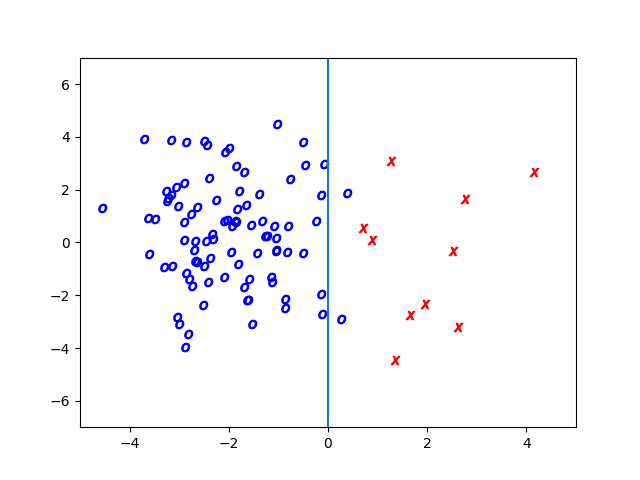
\includegraphics[clip, width=12cm]{../figures/assignment3_result_weighted_train}
    \caption{重み付き,訓練データに対する結果}
    \label{fig:weighted_train}
\end{figure}

\begin{figure}[H]
    \centering
    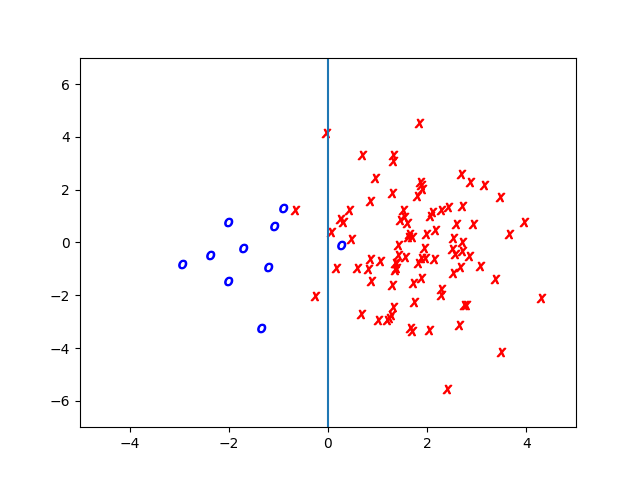
\includegraphics[clip, width=12cm]{../figures/assignment3_result_weighted_test}
    \caption{重み付き,テストデータに対する結果}
    \label{fig:weighted_test}
\end{figure}

\begin{figure}[H]
    \centering
    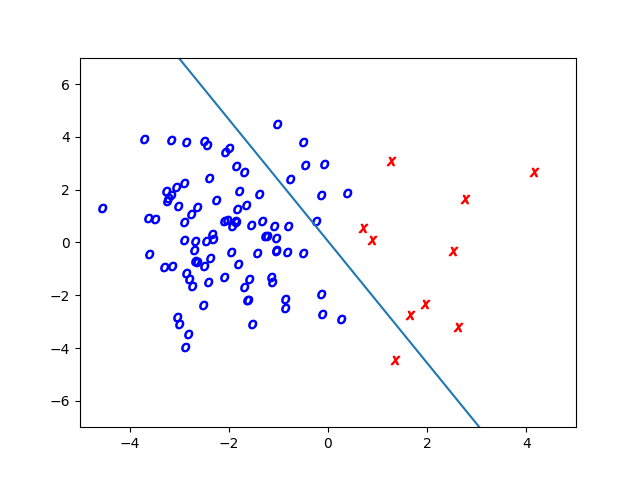
\includegraphics[clip, width=12cm]{../figures/assignment3_result_unweighted_train}
    \caption{重み付けなし,訓練データに対する結果}
    \label{fig:unweighted_train}
\end{figure}

\begin{figure}[H]
    \centering
    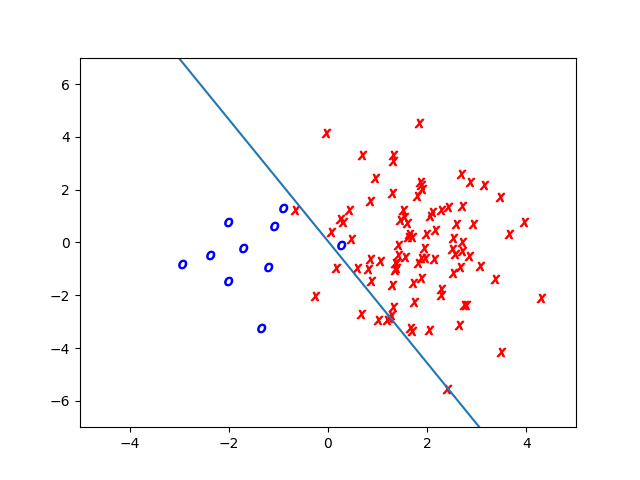
\includegraphics[clip, width=12cm]{../figures/assignment3_result_unweighted_test}
    \caption{重み付けなし,テストデータに対する結果}
    \label{fig:unweighted_test}
\end{figure}



\end{document}
